\documentclass{article}
\usepackage[utf8]{inputenc}
\usepackage{geometry}
 \geometry{
 a4paper,
 total={170mm,257mm},
 left=20mm,
 top=20mm,
 }
\usepackage{graphicx}
\usepackage{titling}
\usepackage{amsmath}
\usepackage{amssymb}
\usepackage{listings, listingsutf8}
\usepackage{xcolor}
\usepackage{hyperref}
\usepackage{tcolorbox}
\usepackage{enumitem}
\usepackage{booktabs} % For better looking tables
\usepackage{float}
\usepackage{todonotes}


% Define language-specific syntax highlighting for Rust
\lstdefinelanguage{Rust}{
  keywords={break, continue, else, for, if, in, loop, match, while, return, as, const, let, move, mut, ref, struct, enum, union, type, impl, dyn, Self, super, trait, where, use, crate, extern, mod, pub, static, unsafe, async, await, try},
  keywordstyle=\color{blue}\bfseries, % Blue for keywords
  ndkeywords={bool, char, f32, f64, i8, i16, i32, i64, isize, str, String, u8, u16, u32, u64, usize, Vec, Option, Result},
  ndkeywordstyle=\color{teal}\bfseries, % Teal for non-default keywords
  identifierstyle=\color{black}, % Black for identifiers
  sensitive=true,
  comment=[l]{//},
  morecomment=[s]{/*}{*/},
  commentstyle=\color{green!70!black}\ttfamily, % Green for comments
  stringstyle=\color{red}\ttfamily, % Red for strings
  morestring=[b]",
  morestring=[b]'''
}

% Global settings for listings
\lstset{
  language=Rust,
  inputencoding=utf8/latin1,
  basicstyle=\ttfamily\small,
  breaklines=true,
  showstringspaces=false,
  tabsize=4,
  frame=tb,
  numbers=left,
  numberstyle=\tiny\color{gray},
  captionpos=b
}

\title{Empirical Comparison of QuickSelect and LazySelect Algorithms}
\author{Charels Hugo}
\date{October 2024}

% Custom header and footer
\usepackage{fancyhdr}
\fancypagestyle{plain}{
    \fancyhf{} % clear all header and footer fields
    \fancyfoot[R]{
\includegraphics[width=2cm]{assets/pictures/ULB.png}}
    \fancyfoot[L]{\today}
    \fancyhead[L]{Assignment 1: Selection}
    \fancyhead[R]{\theauthor}
}

\makeatletter
\def\@maketitle{%
  \newpage
  \null
  \vskip 1em%
  \begin{center}%
  \let \footnote \thanks
    {\LARGE \@title \par}%
    \vskip 1em%
    %{\large \@date}%
  \end{center}%
  \par
  \vskip 1em}
\makeatother

\usepackage{lipsum}
\usepackage{cmbright}

\begin{document}

\maketitle

% Information about the assignment
\noindent\begin{tabular}{@{}ll}
    Student & Charels Hugo \\
    Course  & INFO-F413 \\
    Instructor  & Jean Cardinal
\end{tabular}


\begin{abstract}
This report presents the implementation and empirical comparison of two randomized selection algorithms: QuickSelect and LazySelect. We validate the theoretical number of comparisons through extensive testing on input sizes ranging from \(10^4\) to \(10^7\). The report highlights the implementation details, experimental setup, and conclusions on the efficiency and practical use of each algorithm. Based on our results, LazySelect shows a clear advantage for input sizes larger than two million elements, while QuickSelect performs better on smaller inputs.
\end{abstract}



\section{Introduction}
The selection problem involves finding the \(k\)-th smallest (or largest) element in an unsorted array. QuickSelect is a widely used randomized algorithm for this task, while LazySelect is an optimized variant aimed at reducing the number of comparisons and improving overall efficiency for large datasets.

This report implements, analyzes, and empirically compares these two algorithms, focusing on the number of comparisons, the actual running time, and the number of comparisons depending of \(k\). The latter metric is particularly interesting as it highlights how the efficiency of each algorithm changes with the position of the target element. Our goal is to determine which algorithm is more suitable for different input sizes, with practical recommendations based on the results.



\section{Algorithm Descriptions}

\subsection{QuickSelect}

QuickSelect is a divide-and-conquer algorithm that selects a random pivot, partitions the array, and recursively selects from one partition. The expected number of comparisons is given by:
\[
\mathbb{E}[\text{\#comparisons}] = 2n + 2k \ln\left(\frac{n-k}{k}\right) + 2n \ln\left(\frac{n}{n-k}\right),
\]
which can be approximated asymptotically as \(2n(1 + h(\alpha))\), where \( \alpha = \frac{k}{n} \) and \( h(\alpha) \) is the entropy function describing uncertainty in partitioning. For simplicity, the expected number of comparisons is at most \(2n(1 + \ln{2}) \simeq 3.386n \), providing a straightforward estimation.



\subsection{LazySelect}

LazySelect improves upon QuickSelect by using a sampling-based strategy. It selects a subset of elements and employs two pivots to partition the array, reducing the search space. This method ensures that, with high probability, the algorithm performs only \(2n + o(n)\) comparisons. As a result, LazySelect achieves performance comparable to the best deterministic selection algorithms, which require at least \(3n\) comparisons in the worst case.



\section{Implementation Details}

Both algorithms were implemented in Rust. The QuickSelect implementation follows the pseudocode from \cite{wiki:QuickSelect}, while LazySelect was based on \cite{motwani1995randomized}. Some adjustments were made to correct minor issues and enhance performance. The full source code is included in \hyperref[appendix:code]{Appendix}, where detailed comments and explanations are provided for each part of the implementation.


\section{Experimental Plan}

The experiment is designed to evaluate and compare the performance of QuickSelect and LazySelect by analyzing both the number of comparisons and the execution time. In addition, we will examine how the number of comparisons varies for different \(k\) values within the same list size. All executions are performed on lists of random numbers between 0 and the list size, with \(k\) also chosen randomly within the same range. The plan consists of the following steps:

\begin{itemize}
    \item Implement QuickSelect and LazySelect in Rust.
    \item Track the number of comparisons using a custom `Integer` class that increments a counter for each comparison.
    \item Run both algorithms on input arrays of sizes ranging from \(10^4\) to \(10^7\), with a specific increment to obtain 20 points between the range each time.
    \item Measure the runtime and number of comparisons for each input size.
    \item Perform 100 trials for each input size, averaging the results to obtain reliable data.
    \item Additionally, compare the number of comparisons for value of \(k\) between $0$ and the list size $-1$ within the same input size to observe how the algorithms behave depending on the position of the selected element.
    \item Generate graphs to visualize the relationship between input size, \(k\)-values, number of comparisons, and runtime execution.
    \item Analyze the results and discuss any patterns or deviations from theoretical expectations, particularly focusing on large input sizes and variations in \(k\)-values.
\end{itemize}

\section{Experimental Results}

The following section presents and analyzes the experimental results obtained from running the QuickSelect and LazySelect algorithms on varying list sizes. The experiments focus on two key metrics: the number of comparisons and the runtime (in milliseconds). Additionally, we analyze the number of comparisons based on different \(k\)-values within a fixed list size.

\subsection{Number of Comparisons and Runtime per List Size}

We first compare the number of comparisons and the runtime for varying list sizes, starting from \(n = 5000\) to \(n = 10^7\), with intervals chosen to show the algorithm's performance over both small and large data sets.

\begin{figure}[H]
    \centering
    \begin{minipage}{0.45\textwidth}
        \centering
        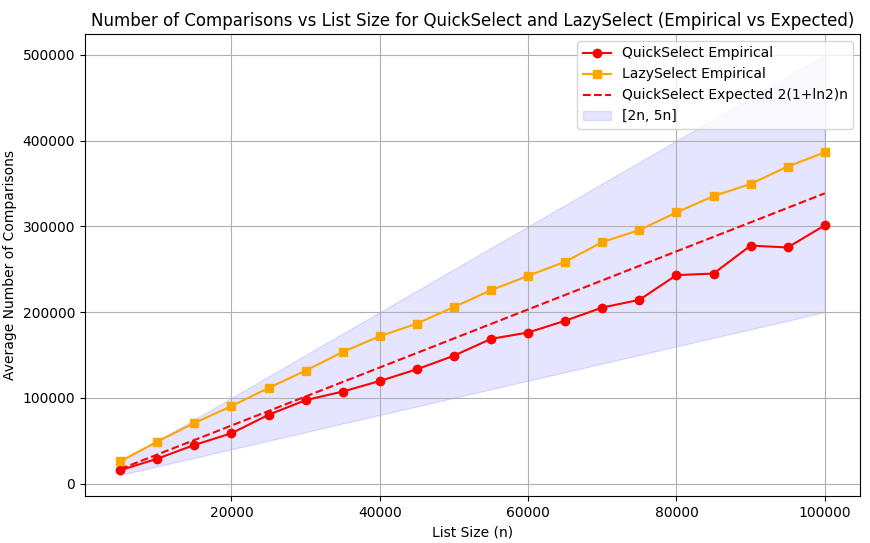
\includegraphics[width=\textwidth]{assets1/graphics/comparisons_results_5000_100000_5000_100.png}
        \caption{Number of comparisons per list size, $n \in [5000, 100000]$}
    \end{minipage}
    \hfill
    \begin{minipage}{0.45\textwidth}
        \centering
        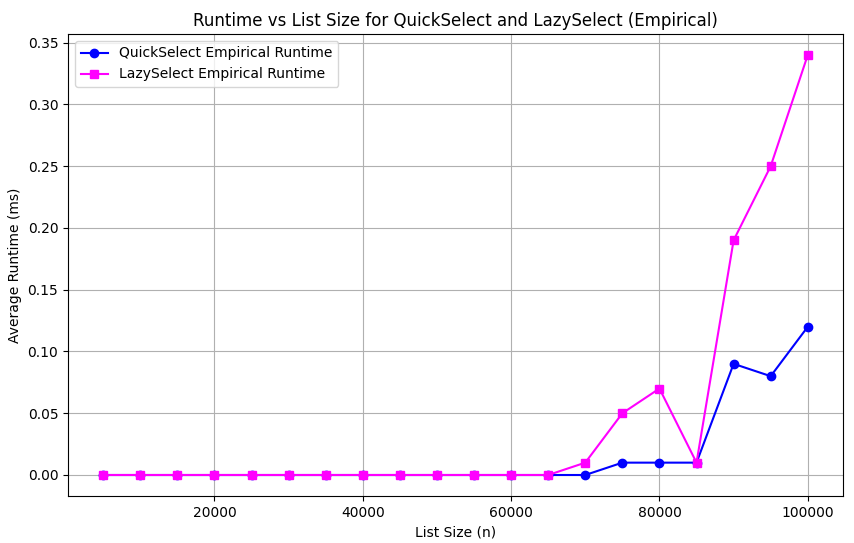
\includegraphics[width=\textwidth]{assets1/graphics/runtime_results_5000_100000_5000_100.png}
        \caption{Runtime (ms) per list size, $n \in [5000, 100000]$}
    \end{minipage}
\end{figure}

\noindent In the first pair of graphs, for smaller input sizes (\(5000 \leq n \leq 100000\)):
\begin{itemize}
    \item The **number of comparisons** increases linearly as the list size grows. This aligns with the expected behavior for both QuickSelect and LazySelect, where comparisons scale with \(O(n)\). In this range, we observe that the growth in comparisons is more than \(2n\) but less than \(5n\), confirming the linear complexity.
    \item The **runtime** for these sizes remains nearly constant up to a list size of \(n = 70000\), due to Rust’s efficient compilation and optimizations at the O3 level. Beyond this size, the runtime begins to increase.
\end{itemize}

\begin{figure}[H]
    \centering
    \begin{minipage}{0.45\textwidth}
        \centering
        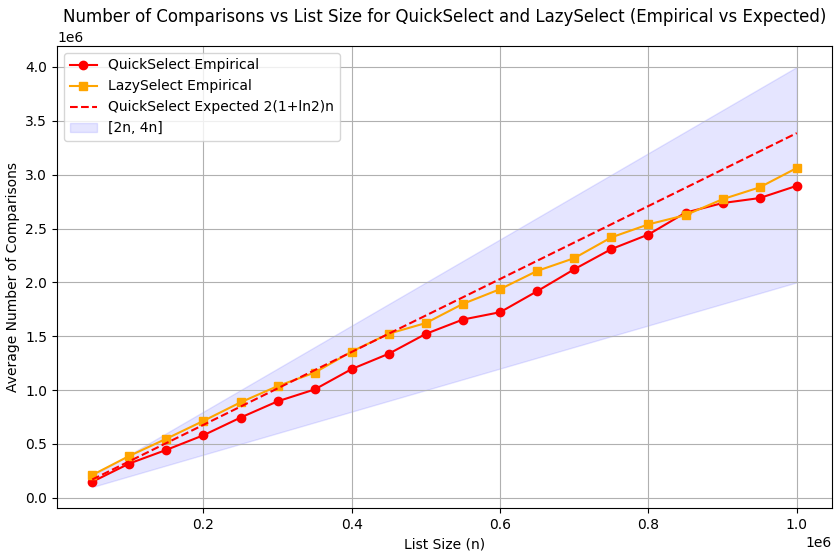
\includegraphics[width=\textwidth]{assets1/graphics/comparisons_results_50000_1000000_50000_100.png}
        \caption{Number of comparisons per list size, $n \in [50000, 1000000]$}
    \end{minipage}
    \hfill
    \begin{minipage}{0.45\textwidth}
        \centering
        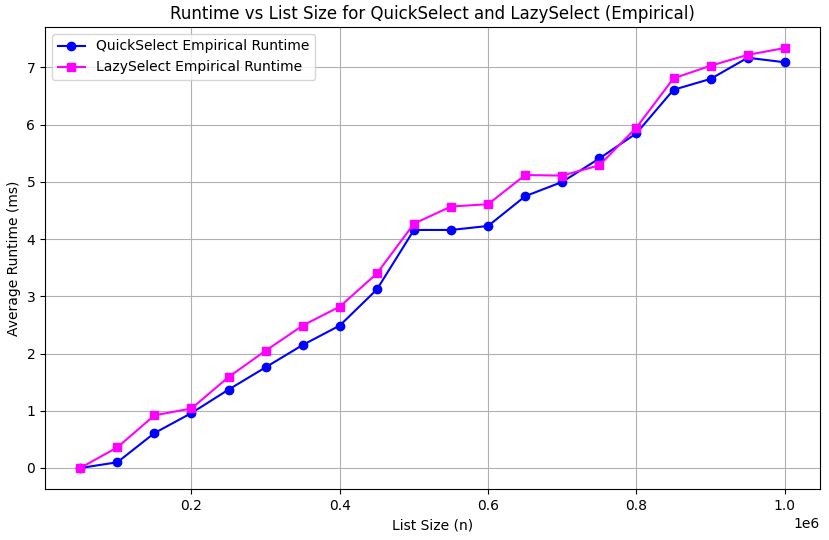
\includegraphics[width=\textwidth]{assets1/graphics/runtime_results_50000_1000000_50000_100.png}
        \caption{Runtime (ms) per list size, $n \in [50000, 1000000]$}
    \end{minipage}
\end{figure}

\noindent For **medium-sized lists** (\(50000 \leq n \leq 10^6\)):
\begin{itemize}
    \item The **number of comparisons** continues to show linear scaling, but the range decreases compared to smaller sizes, now falling between \(2n\) and \(4n\).
    \item The **runtime** curve mirrors the comparison results, increasing consistently as the list size grows larger.
\end{itemize}

\begin{figure}[H]
    \centering
    \begin{minipage}{0.45\textwidth}
        \centering
        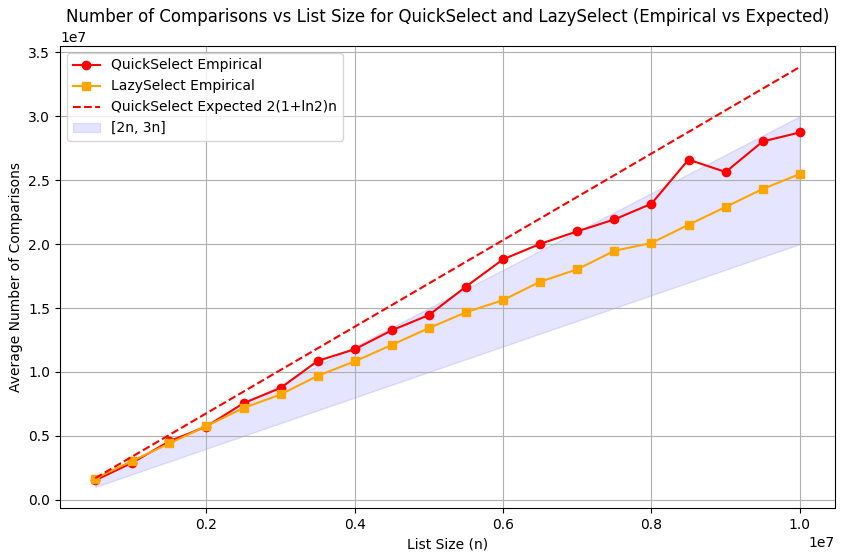
\includegraphics[width=\textwidth]{assets1/graphics/comparisons_results_500000_10000000_500000_100.png}
        \caption{Number of comparisons per list size, $n \in [500000, 10000000]$}
    \end{minipage}
    \hfill
    \begin{minipage}{0.45\textwidth}
        \centering
        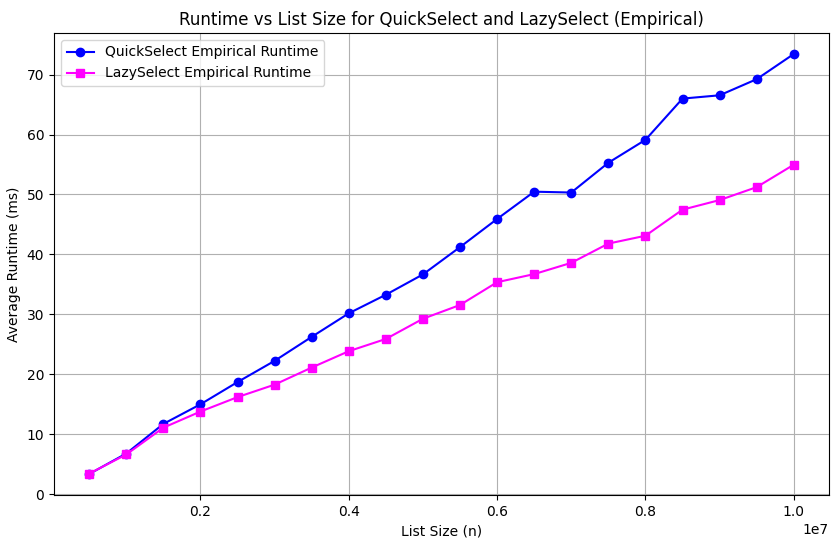
\includegraphics[width=\textwidth]{assets1/graphics/runtime_results_500000_10000000_500000_100.png}
        \caption{Runtime (ms) per list size, $n \in [500000, 10000000]$}
    \end{minipage}
\end{figure}

\noindent For **large lists** (\(n = 5 \times 10^5\) to \(n = 10^7\)):
\begin{itemize}
    \item The **number of comparisons** shows that LazySelect outperforms QuickSelect, with the number of comparisons now ranging between \(2n\) and \(3n\), significantly better than QuickSelect’s higher comparison counts.
    \item The **runtime** follows the same trend, with LazySelect running faster than QuickSelect for these larger list sizes.
\end{itemize}

These results suggest that LazySelect becomes the more efficient algorithm for large input sizes, both in terms of the number of comparisons and runtime, while QuickSelect is better suited for smaller lists due to its lower overhead.

\subsection{Number of Comparisons for Each Value of \(k\)}

In this section, we investigate how the number of comparisons varies with different values of \(k\), which represents the rank of the element to be selected in the list.

\begin{figure}[H]
    \centering
    \begin{minipage}{0.45\textwidth}
        \centering
        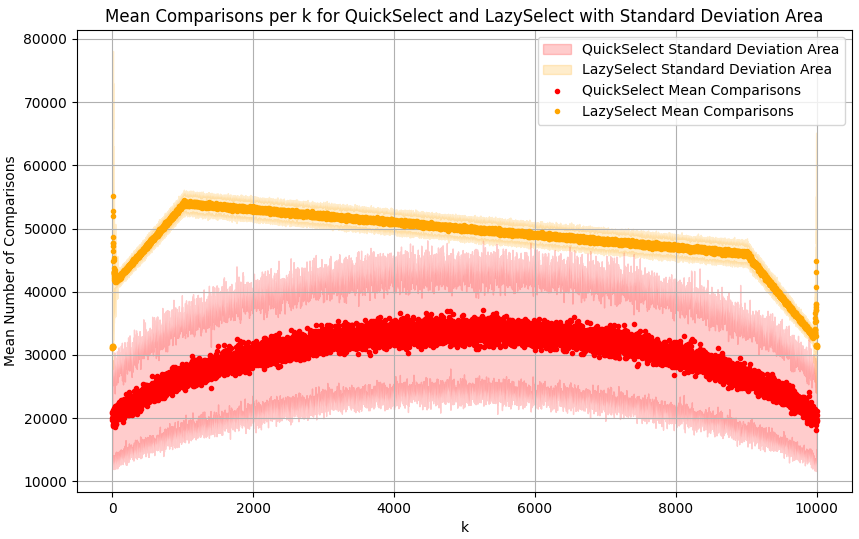
\includegraphics[width=\textwidth]{assets1/graphics/comparisons_results_k_10000_100.png}
        \caption{Number of comparisons per $k$, $n = 10000$ and $k \in [0, 10000]$}
    \end{minipage}
    \hfill
    \begin{minipage}{0.45\textwidth}
        \centering
        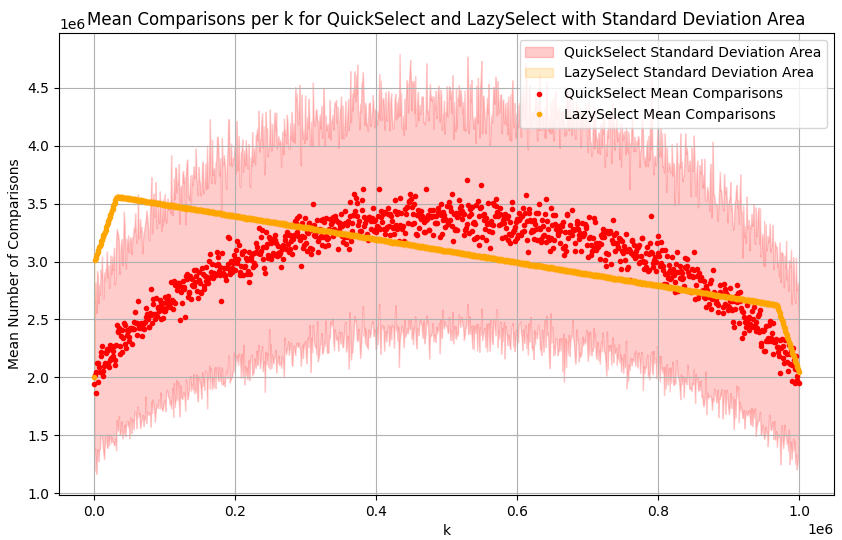
\includegraphics[width=\textwidth]{assets1/graphics/comparisons_results_k_1000000_100.png}
        \caption{Number of comparisons per $k$, $n = 1000000$ and $k \in [0, 1000000]$}
    \end{minipage}
\end{figure}

The results show that for LazySelect, the number of comparisons is highest when \(k\) is near the median, and decreases as \(k\) approaches the extremum values, i.e., near \(k = 0\) or \(k = n\). LazySelect displays a completely different behavior from QuickSelect, one that would be interesting to explore further and analyze in depth. However, this is beyond the scope of this report. Additionally, QuickSelect has a larger standard deviation in the number of comparisons compared to LazySelect, which maintains almost no standard deviation across different values of \(k\). 

\section{Discussion}

The experimental results demonstrate a clear relationship between the input size and the efficiency of QuickSelect and LazySelect. For smaller list sizes, QuickSelect performs better due to its lower overhead and fewer constant factors, making it faster in practice. However, as the list size increases, LazySelect surpasses QuickSelect, thanks to its improved sampling strategy and fewer overall comparisons.

For each value of \(k\), we observe that QuickSelect's performance is particularly interesting. It requires the highest number of comparisons when selecting elements near the median of the list, and this number decreases as \(k\) approaches the extremum values. QuickSelect also shows a greater variance in its performance compared to LazySelect, which maintains a much more stable number of comparisons regardless of \(k\).

Despite the additional overhead in sampling, the runtime results indicate that LazySelect's overall performance is not negatively impacted. The runtime curves align closely with the comparison curves, suggesting that the sampling process does not introduce a significant penalty, further emphasizing LazySelect’s efficiency in larger datasets.

These results suggest that LazySelect has distinct advantages, especially for large datasets, as it minimizes comparisons more effectively than QuickSelect. Its unique behavior when \(k\) is near the extremum values presents a potential for further study, but that is not the focus of this report.

\section{Conclusion}

In this report, we have implemented and empirically compared two randomized selection algorithms: QuickSelect and LazySelect. Our experiments validate the theoretical performance claims for both algorithms. QuickSelect performs efficiently for smaller datasets, while LazySelect outperforms QuickSelect for larger lists, with the tipping point occurring around two million elements.

These findings offer practical guidance on selecting the appropriate algorithm depending on the dataset size and the specific requirements of the task. LazySelect is particularly advantageous when large datasets or a significant reduction in comparisons is needed. Future work could extend this analysis to other selection algorithms and explore further optimizations within LazySelect.





\bibliographystyle{plain}
\bibliography{references}

\newpage

\appendix
\section{Source Code}

\label{appendix:code}
\subsection{QuickSelect Implementation}
\lstinputlisting[language=Rust, caption=QuickSelect]{assets1/code/quickselect.rs}

\subsection{LazySelect Implementation}
\lstinputlisting[language=Rust, caption=LazySelect]{assets1/code/lazyselect.rs}

\subsection{Integer Class Implemenation}
\lstinputlisting[language=Rust, caption=LazySelect]{assets1/code/integer.rs}


\end{document}
